\documentclass{beamer}
\usepackage{amsfonts,amsmath,oldgerm}
\usetheme{dmpisa} % Here the call to the beamer theme

\usepackage[english]{babel}
\usepackage{hyperref}
\usepackage{media9}
\usepackage{multimedia}
\usepackage{graphicx}
\usepackage{animate}
\usepackage{subfig}
%\usepackage{enumitem}
\usepackage[font=scriptsize]{caption}
\captionsetup[subfigure]{labelformat=empty}



%Per stile dei teoremi, delle definizioni, etc...
\theoremstyle{definition}
\newtheorem{dfn}{Definizione}[section]
\newtheorem{es}{Esempio}[section]
\newtheorem{oss}{Osservazione}[section]
\newtheorem{ese}{Esercizio}[section]
\theoremstyle{plain}
\newtheorem{thm}{Teorema}[section]
\newtheorem{cor}{Corollario}[section]
\newtheorem{lem}{Lemma}[section]
\newtheorem{prop}{Proposizione}[section]

%%
\newcommand{\testcolor}[1]{\colorbox{#1}{\textcolor{#1}{test}}~\texttt{#1}}
\usefonttheme[onlymath]{serif}
\titlebackground*{assets/background}
\newcommand{\hrefcol}[2]{\textcolor{cyan}{\href{#1}{#2}}}

\title{HLT Project: Progress Update}
\subtitle{Sentiment Analysis on Amazon Reviews}
\vspace{0.3cm}
\course{HLT - Group 11}
%\vspace{0.3cm}
\author{\href{mailto:a.nardone5@studenti.unipi.it}{Angelo Nardone}, \href{mailto:r.marcaccio@studenti.unipi.it}{Riccardo Marcaccio}, \href{mailto: m.ziboli@studenti.unipi.it}{Matteo Ziboli}}
\date{May 20, 2024}

\begin{document}
\maketitle

\footlinecolor{maincolor}

%~~~~~~~~~~~~~~~~~~~~~~~~~~~~~~~~~~~~~~~~~~~~~~~~~~~~~~~~~~~~~~~~~~~~~~~~~
\begin{frame}{Introduction}
\framesubtitle{HLT Project: Progress Update}
{\small 
\begin{itemize}
    \item Previous presentation: explored and cleaned the data we worked with.
    \item Recall that the data represents "Amazon Reviews."
    \item Used this data to address two main tasks, which we'll analyze today.
    \item Specifically, the tasks we'll cover are:
    \begin{enumerate}
        \item \textbf{Classification (Sentiment Analysis).}
        \item \textbf{Negative Reviews Categorization.}
    \end{enumerate}
\end{itemize}
}
\end{frame}

%~~~~~~~~~~~~~~~~~~~~~~~~~~~~~~~~~~~~~~~~~~~~~~~~~~~~~~~~~~~~~~~~~~~~~~~~~~~~~~~~~~~~~
\section{Classification}

%~~~~~~~~~~~~~~~~~~~~~~~~~~~~~~~~~~~~~~~~~~~~~~~~~~~~~~~~~~~~~~~~~~~~~~~~~
\begin{frame}{Introduction}
\framesubtitle{HLT Project: Classification}
{\small 
\begin{itemize}
\item The goal is to determine whether a review is negative (label=0) or positive (label=1) based only on the title.
\item It's a \textbf{supervised task} type: we have correct labels to train the model on.
\item Used 80\% of the data for train and 20\% for test. 
\item Analyze the results obtained using various models, starting from simpler models and progressing to more complex ones.
\end{itemize}
}
\end{frame}

%~~~~~~~~~~~~~~~~~~~~~~~~~~~~~~~~~~~~~~~~~~~~~~~~~~~~~~~~~~~~~~~~~~~~~~~~~
\begin{frame}{Lexicon with VADER}
\framesubtitle{HLT Project: Classification}

\begin{columns}
    \column{0.5\textwidth}
    \vspace{-1cm}
    {\small 
        \begin{itemize}
        \item Used \textcolor{teal}{VADER} (Valence Aware Dictionary and sEntiment Reasoner) for the first model.
        \item VADER is a \textbf{lexicon} and sentiment analysis tool integrated into \textcolor{teal}{NLTK} (Natural Language Toolkit).
        \item Achieved an accuracy of 67\%. 
        \item Difficulty in detecting negative reviews.
        \end{itemize}
    }

    \column{0.5\textwidth}
    \vspace{-0.3cm}
    \begin{figure}
        \centering
        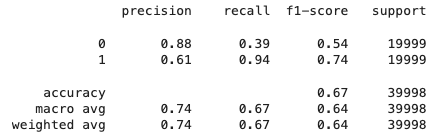
\includegraphics[scale=0.4]{Figures/lexicon_acc.png}
    \end{figure}
    \vspace{-0.3cm}
    \begin{figure}
        \centering
        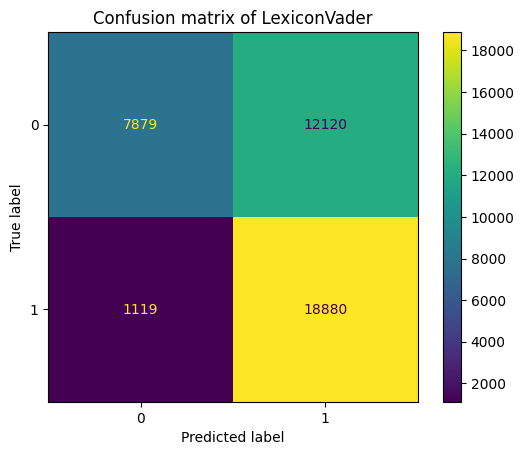
\includegraphics[scale=0.35]{Figures/Lexicon.png}
    \end{figure}
\end{columns}
\end{frame}

%~~~~~~~~~~~~~~~~~~~~~~~~~~~~~~~~~~~~~~~~~~~~~~~~~~~~~~~~~~~~~~~~~~~~~~~~~
\begin{frame}{Multinomial Naive Bayes}
\framesubtitle{HLT Project: Classification}

\begin{columns}
    \column{0.5\textwidth}
    \vspace{-1cm}
    {\small 
        \begin{itemize}
            \item For second classifier, used \textbf{Multinomial Naive Bayes}.
            \item To extract information from textual data, used \textcolor{teal}{CountVectorizer} and \textcolor{teal}{SelectKBest}.
            \item Achieved an accuracy of 81\%.
            \item Much more balance in predicting positive and negative classes.
        \end{itemize}
    }

    \column{0.5\textwidth}
    \vspace{-0.3cm}
    \begin{figure}
        \centering
        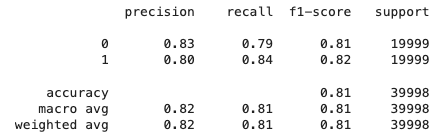
\includegraphics[scale=0.4]{Figures/naive_bayes_acc.png}
    \end{figure}
    \vspace{-0.3cm}
    \begin{figure}
        \centering
        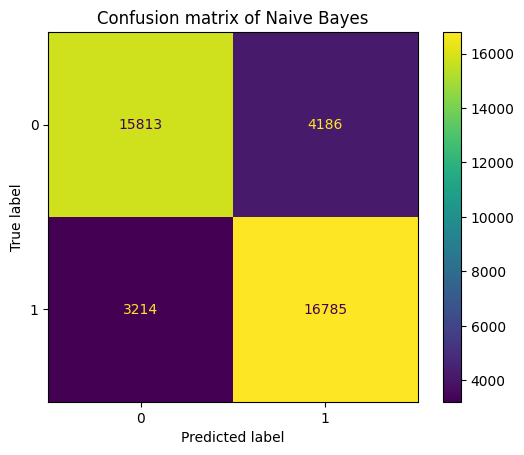
\includegraphics[scale=0.35]{Figures/NaiveBayes.png}
    \end{figure}
\end{columns}
\end{frame}

%~~~~~~~~~~~~~~~~~~~~~~~~~~~~~~~~~~~~~~~~~~~~~~~~~~~~~~~~~~~~~~~~~~~~~~~~~
\begin{frame}{Multi-Layer Perceptron}
\framesubtitle{HLT Project: Classification}

\begin{columns}
    \column{0.5\textwidth}
    \vspace{-1cm}
    {\small 
        \begin{itemize}
            \item Also used a simple \textbf{Multi-Layer Perceptron}, with \textcolor{teal}{MLPClassifier} from \textcolor{teal}{sklearn}.
            \item Same operations for extract information from textual data.
            \item Achieved an accuracy of 83\%.
            \item Best results among the models seen so far.
        \end{itemize}
    }

    \column{0.5\textwidth}
    \vspace{-0.3cm}
    \begin{figure}
        \centering
        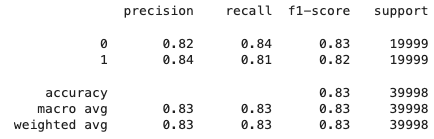
\includegraphics[scale=0.4]{Figures/MLP-acc.png}
    \end{figure}
    \vspace{-0.3cm}
    \begin{figure}
        \centering
        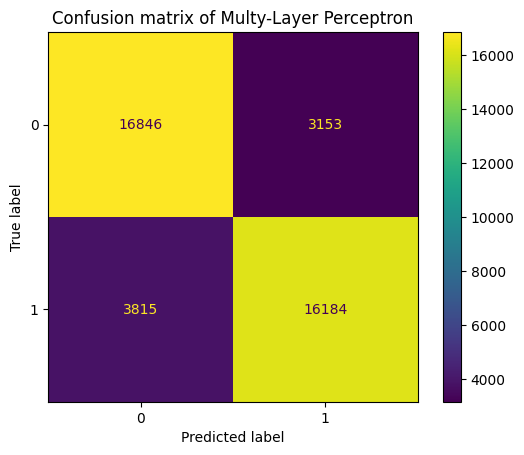
\includegraphics[scale=0.35]{Figures/MultyLayer Perceptron.png}
    \end{figure}
\end{columns}
\end{frame}

%~~~~~~~~~~~~~~~~~~~~~~~~~~~~~~~~~~~~~~~~~~~~~~~~~~~~~~~~~~~~~~~~~~~~~~~~~
\begin{frame}{LLM using Bert}
\framesubtitle{HLT Project: Classification}
{\small
\vspace{-0.1cm}
\begin{itemize}
    \item Final Model: Using a Large Language Model (LLM).
    \item Used \textcolor{teal}{BERT-base-cased} to \textbf{tokenize} and \textbf{generate embeddings} for each sentence.
    \item A three-layer feedforward neural network is applied for classification.
\end{itemize}
}

\begin{figure}
    \centering
    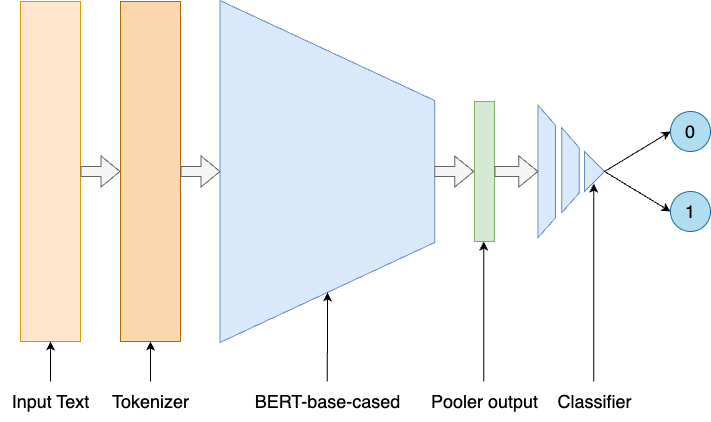
\includegraphics[scale=0.3]{Figures/Model.png}
\end{figure}
\end{frame}

%~~~~~~~~~~~~~~~~~~~~~~~~~~~~~~~~~~~~~~~~~~~~~~~~~~~~~~~~~~~~~~~~~~~~~~~~~
\begin{frame}{LLM using Bert}
\framesubtitle{HLT Project: Classification}
{\small
\vspace{-0.1cm}
\begin{itemize}
    \item<1-> Used a dual phase for training.
    \item<1-> Initially trained all the parameters: \textbf{fine-tuning}.
    \item<2-> During final epochs, trained only the feedforward classifier, keeping the \textbf{Bert weights frozen}.
\end{itemize}
}

\begin{figure}
    \centering
    \only<1>{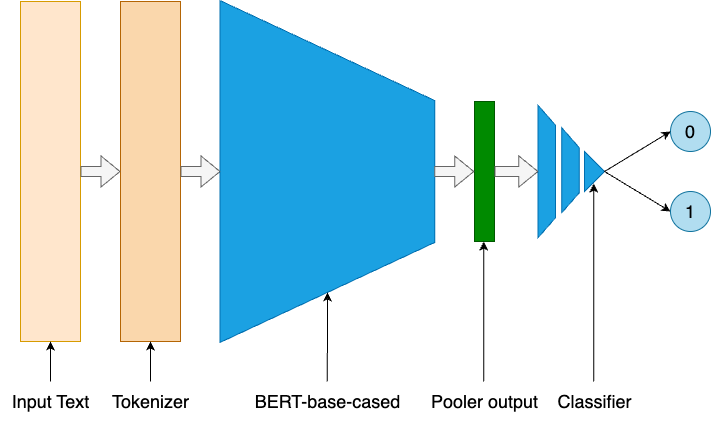
\includegraphics[scale=0.3]{Figures/Modello3.png}}
    \only<2>{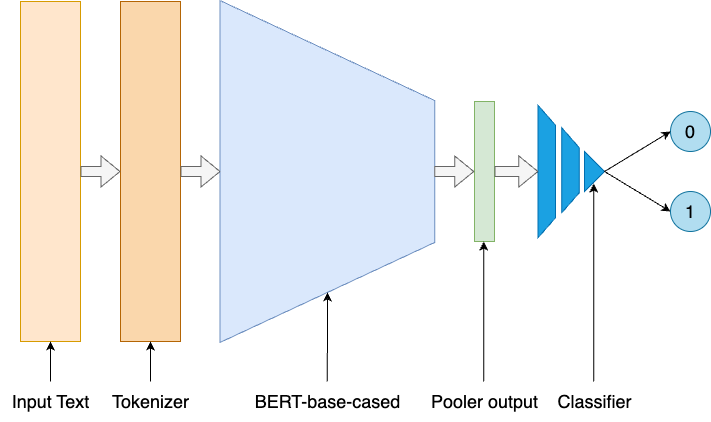
\includegraphics[scale=0.3]{Figures/Modello2.png}}
\end{figure}
\end{frame}

%~~~~~~~~~~~~~~~~~~~~~~~~~~~~~~~~~~~~~~~~~~~~~~~~~~~~~~~~~~~~~~~~~~~~~~~~~
\begin{frame}{LLM using Bert}
\framesubtitle{HLT Project: Classification}

\begin{columns}
    \column{0.5\textwidth}
    \vspace{-1cm}
    {\small 
        \begin{itemize}
            \item For now still few tests with this model, exploring few hyperparameters.
            \item Achieved an accuracy of 91\%.
            \item Improvement over all previous models.
        \end{itemize}
    }

    \column{0.5\textwidth}
    \vspace{-0.3cm}
    \begin{figure}
        \centering
        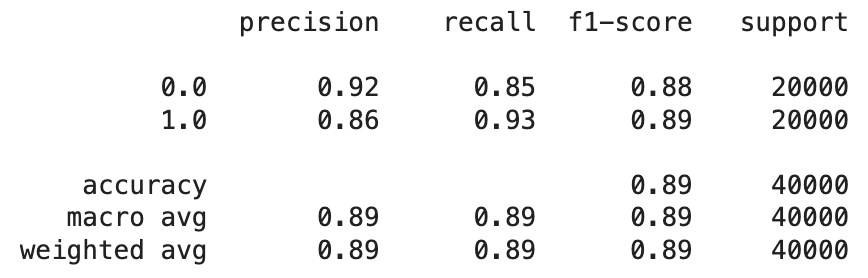
\includegraphics[scale=0.4]{Figures/classifier_acc.png}
    \end{figure}
    \vspace{-0.3cm}
    \begin{figure}
        \centering
        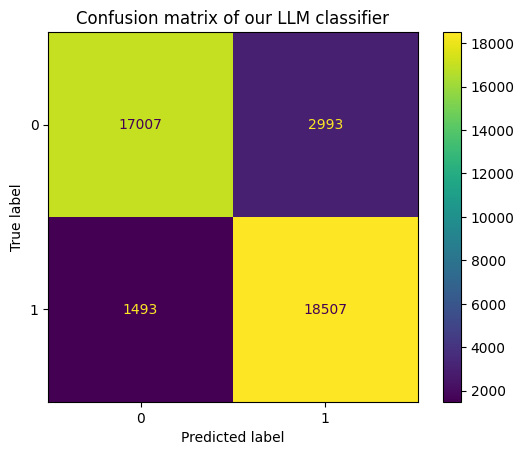
\includegraphics[scale=0.35]{Figures/classifier.png}
    \end{figure}
\end{columns}
\end{frame}

%~~~~~~~~~~~~~~~~~~~~~~~~~~~~~~~~~~~~~~~~~~~~~~~~~~~~~~~~~~~~~~~~~~~~~~~~~~~~~~~~~~~~~
\section{Negative Reviews Categorization}

\begin{frame}{Introduction}
\framesubtitle{HLT Project: Negative Reviews Categorization}
{\small
\begin{itemize}
    \item This task originates from the following question:
    \begin{center}
    \emph{It is possible determine if a negative review is due to delivery times, potential damage, product quality, or other factors?}
    \end{center}
    \item Knowing the answer to this question could be very useful for companies selling products.
    \item Answer this question by using only the negative reviews from the dataset used so far.
    \item This is an \textbf{unsupervised task}: we do not have labels to associate with the data.
\end{itemize}
}
\end{frame}


%~~~~~~~~~~~~~~~~~~~~~~~~~~~~~~~~~~~~~~~~~~~~~~~~~~~~~~~~~~~~~~~~~~~~~~~~~
\begin{frame}{Clustering on Embedding Vectors}
\framesubtitle{HLT Project: Negative Reviews Categorization}
{\small
\begin{itemize}
\item First step: cluster negative reviews by grouping similar ones together.
\item Created a dataset: each title is associated with its \textbf{embedding vector} generated by Bert.
\end{itemize}
}

\begin{figure}
\centering
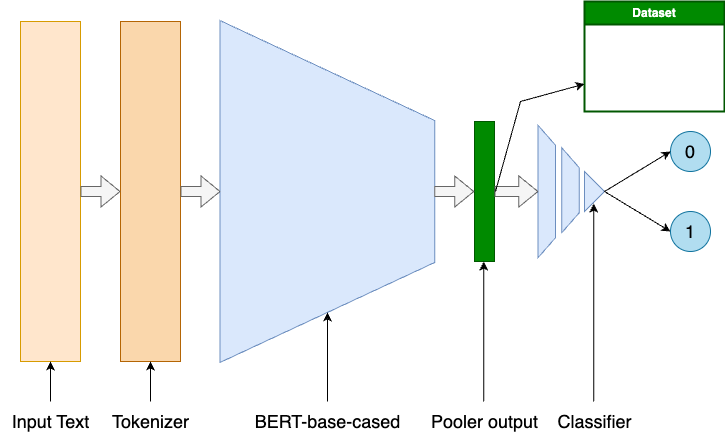
\includegraphics[scale=0.3]{Figures/Modello5.png}
\end{figure}

\end{frame}

%~~~~~~~~~~~~~~~~~~~~~~~~~~~~~~~~~~~~~~~~~~~~~~~~~~~~~~~~~~~~~~~~~~~~~~~~~
\begin{frame}{Clustering on Embedding Vectors}
\framesubtitle{HLT Project: Negative Reviews Categorization}
{\small

\begin{columns}
    \column{0.5\textwidth}
    \begin{itemize}
        \item Considered only the embedding vectors associated with negative titles.
        \item Performed clustering on these using \textcolor{teal}{K-Means}.
        \item Used the \textbf{Elbow Method} to determine the optimal number of clusters.
        \item We chose 2 as the number of clusters.
    \end{itemize}

    \column{0.5\textwidth}
    \begin{figure}
        \centering
        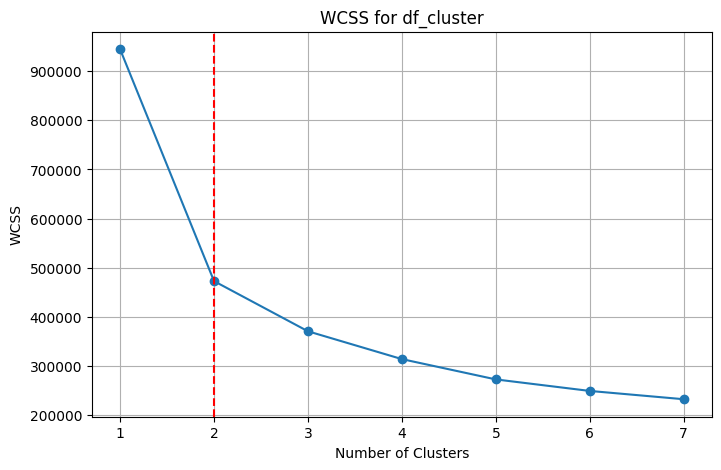
\includegraphics[scale=0.35]{Figures/elbow1.png}
    \end{figure}
\end{columns}
}
\end{frame}

%~~~~~~~~~~~~~~~~~~~~~~~~~~~~~~~~~~~~~~~~~~~~~~~~~~~~~~~~~~~~~~~~~~~~~~~~~
\begin{frame}{Frequent Words}
\framesubtitle{HLT Project: Negative Reviews Categorization}
{\small
\begin{itemize}
    \item To capture the main topics of each cluster, counted the most frequent words in them.
    \item \textbf{Tokenized} each title, removing stopwords and punctuation symbols.
    \item Used methods from \textcolor{teal}{NLTK} to achieve this.
    \item Then counted the number of occurrences in each cluster.
\end{itemize}
}
\end{frame}

%~~~~~~~~~~~~~~~~~~~~~~~~~~~~~~~~~~~~~~~~~~~~~~~~~~~~~~~~~~~~~~~~~~~~~~~~~
\begin{frame}{Results}
\framesubtitle{HLT Project: Negative Reviews Categorization}
{\small 
\begin{columns}
    \column{0.5\textwidth}
    \begin{itemize}
        \item The results obtained were not significant.
        \item Most of the frequent words were common and not indicative of possible topics.
        \item Attributed this result to the fact that used only the titles.
    \end{itemize}
    
    \column{0.5\textwidth}
    \vspace{-0.5cm}
    \begin{figure}
        \centering
        \only<1>{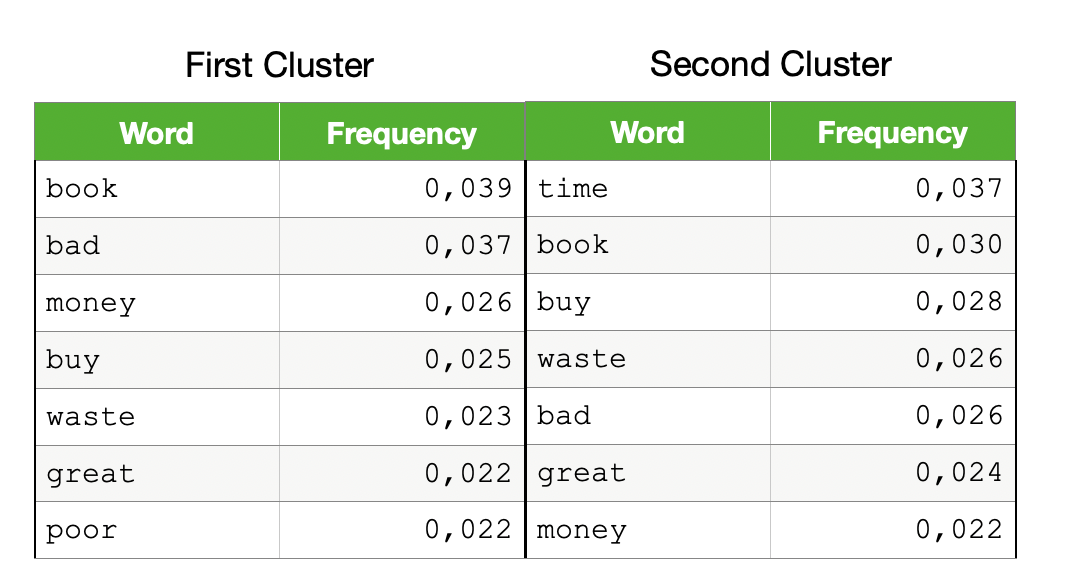
\includegraphics[scale=0.4]{Figures/result1.png}}
        \only<2>{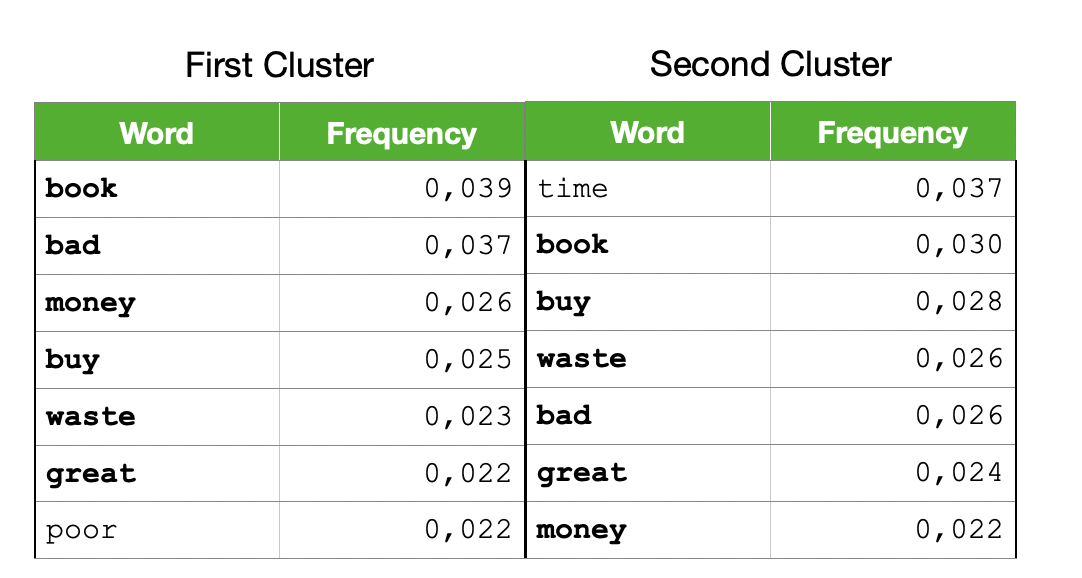
\includegraphics[scale=0.4]{Figures/results2.png}}
    \end{figure}
\end{columns}
}
\end{frame}

%~~~~~~~~~~~~~~~~~~~~~~~~~~~~~~~~~~~~~~~~~~~~~~~~~~~~~~~~~~~~~~~~~~~~~~~~~
\begin{frame}{Embedding Vectors with Word2Vec}
\framesubtitle{HLT Project: Negative Reviews Categorization}
{\small
\begin{itemize}
    \item Attempted the same task but on the entire review texts.
    \item Didn't have the embedding vectors provided by Bert for these texts.
    \item Generated embeddings for the reviews using \textcolor{teal}{Word2Vec}.
    \item For each review, derived an embedding vector by averaging the embedding vectors of all its constituent words (excluding stopwords).
\end{itemize}
}
\end{frame}

%~~~~~~~~~~~~~~~~~~~~~~~~~~~~~~~~~~~~~~~~~~~~~~~~~~~~~~~~~~~~~~~~~~~~~~~~~
\begin{frame}{Clustering on Word2Vec Vectors}
\framesubtitle{HLT Project: Negative Reviews Categorization}
{\small

\begin{columns}
    \column{0.5\textwidth}
    \begin{itemize}
        \item Performed clustering on these using \textcolor{teal}{K-Means}.
        \item Used the \textbf{Elbow Method} to determine the optimal number of clusters.
        \item Again, 2 was the optimal number of clusters.
        \item Used the same methods as before to count words frequency in clusters.
    \end{itemize}

    \column{0.5\textwidth}
    \begin{figure}
        \centering
        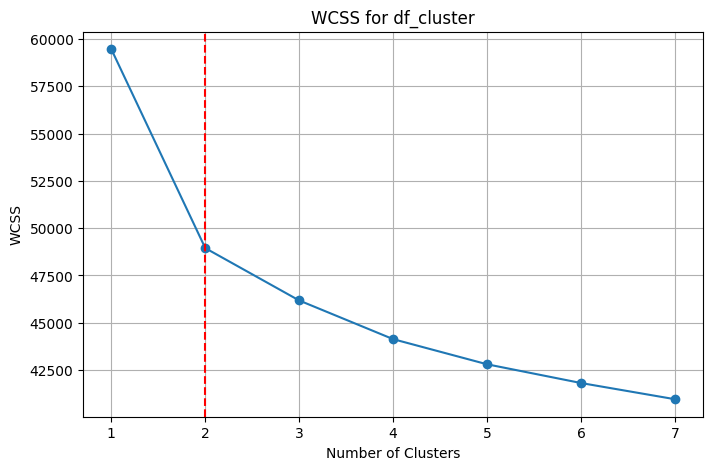
\includegraphics[scale=0.35]{Figures/elbow2.png}
    \end{figure}
\end{columns}
}
\end{frame}

%~~~~~~~~~~~~~~~~~~~~~~~~~~~~~~~~~~~~~~~~~~~~~~~~~~~~~~~~~~~~~~~~~~~~~~~~~
\begin{frame}{Results}
\framesubtitle{HLT Project: Negative Reviews Categorization}
{\small 
    \begin{columns}
    \column{0.5\textwidth}
    \begin{itemize}
        \item Good Result: there are two clearly distinct topics in the two clusters.
            \item First cluster: negative review due to the \textbf{consumer's personal preferences}.
            \begin{itemize}
                \item A product is not visually appealing or artistically satisfying.
                \item A product did not meet the reviewer’s personal taste or expectations regarding content quality.
            \end{itemize}
    \end{itemize}

    \column{0.5\textwidth}
    \vspace{-0.7cm}
    \begin{figure}
        \centering
        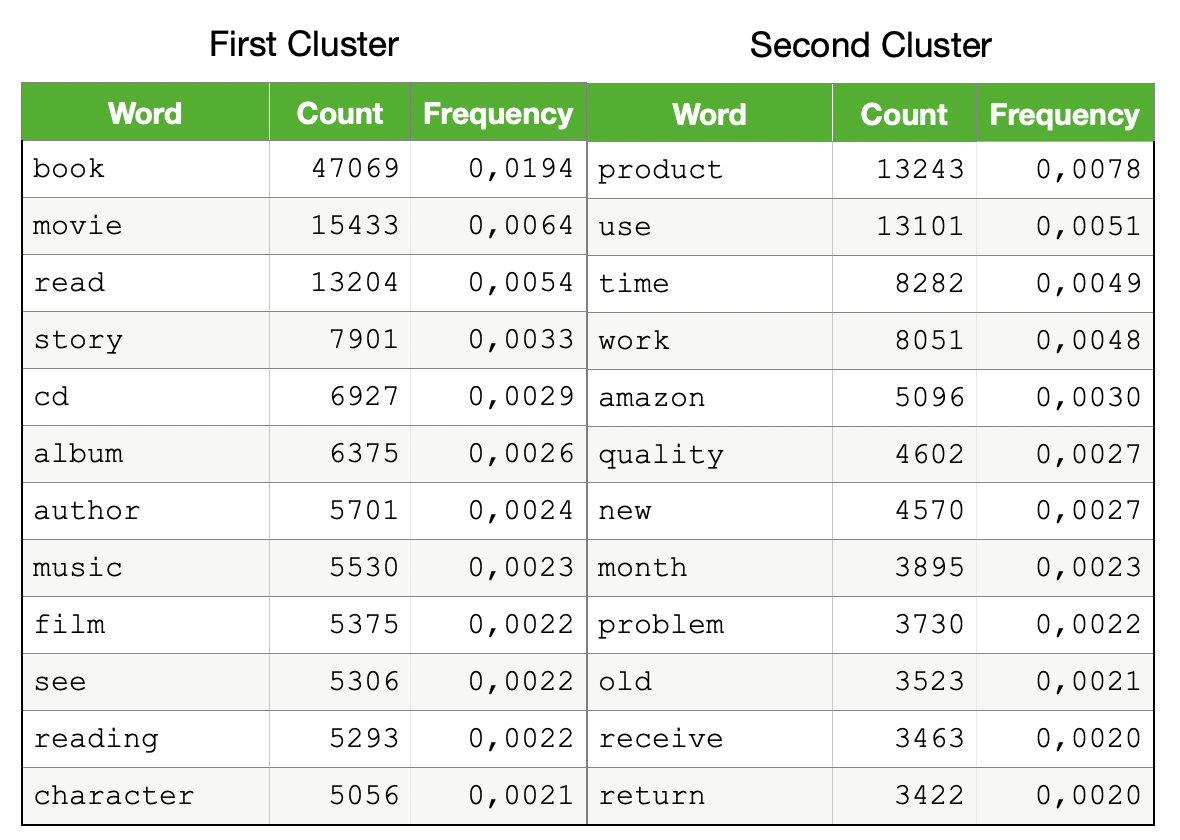
\includegraphics[scale=0.35]{Figures/tabella.png}
    \end{figure}
    \end{columns}
}
\end{frame}

%~~~~~~~~~~~~~~~~~~~~~~~~~~~~~~~~~~~~~~~~~~~~~~~~~~~~~~~~~~~~~~~~~~~~~~~~~
\begin{frame}{Results}
\framesubtitle{HLT Project: Negative Reviews Categorization}
{\small 
    \begin{columns}
    \column{0.5\textwidth}
    \begin{itemize}
        \item Good Result: there are two clearly distinct topics in the two clusters.
            \item Second cluster: many more words suggesting much more \textbf{objective issues}.
            \begin{itemize}
                \item Delivery delays
                \item Physical damage or defects in the product.
            \end{itemize}
    \end{itemize}

    \column{0.5\textwidth}
    \vspace{-0.7cm}
    \begin{figure}
        \centering
        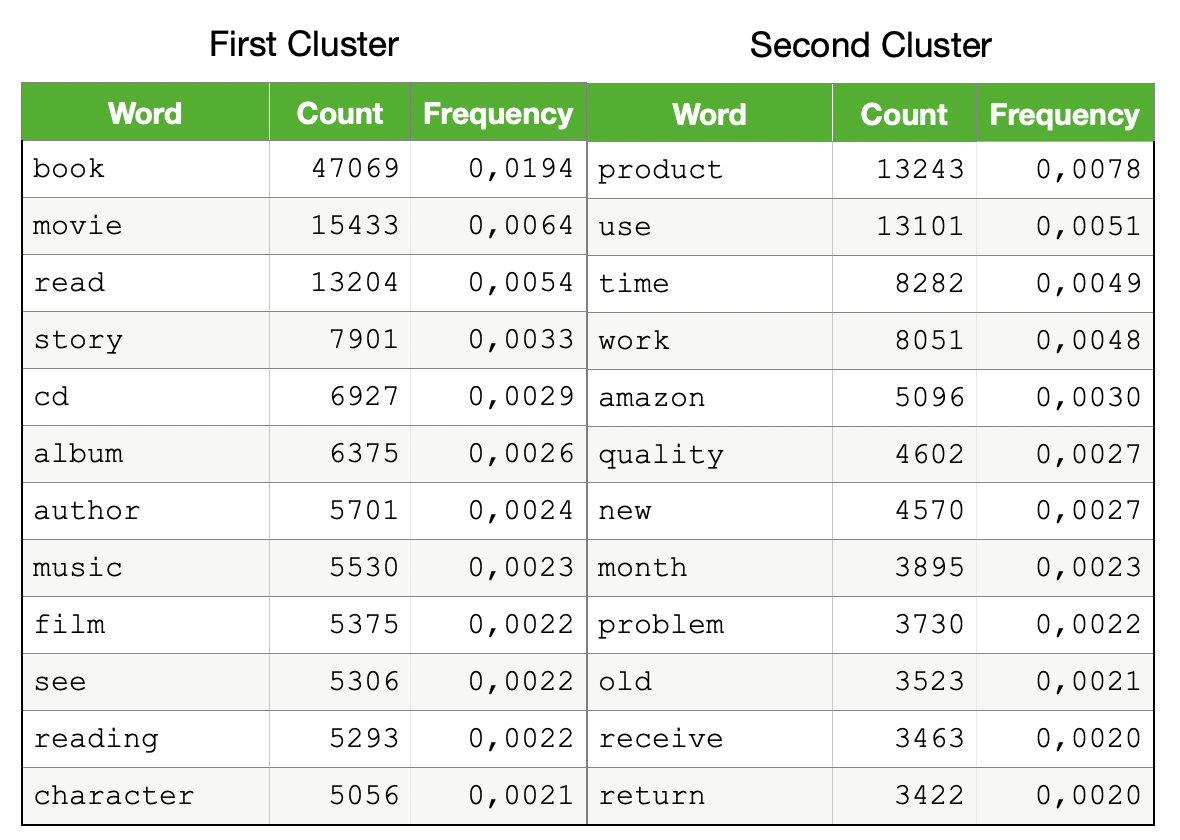
\includegraphics[scale=0.35]{Figures/tabella.png}
    \end{figure}
    \end{columns}
}
\end{frame}


%~~~~~~~~~~~~~~~~~~~~~~~~~~~~~~~~~~~~~~~~~~~~~~~~~~~~~~~~~~~~~~~~~~~~~~~~~~~~~~~~~~~~~
\section{Conclusion}

%~~~~~~~~~~~~~~~~~~~~~~~~~~~~~~~~~~~~~~~~~~~~~~~~~~~~~~~~~~~~~~~~~~~~~~~~~
\begin{frame}{Overview}
\framesubtitle{HLT Project: Expanding Model Insights}
{\small
\begin{itemize}
    \item Achieved good results for the tasks presented.
    \item However, our goal by the end of May is to:
    \begin{enumerate}
        \item Improve the obtained results through further experimentation.
        \item See the results of Negative Reviews Categorization using Bert on whole reviews.
        \item Explore new methods and tasks where there is potential for interesting findings.
    \end{enumerate}
\end{itemize}
}
\end{frame}


%~~~~~~~~~~~~~~~~~~~~~~~~~~~~~~~~~~~~~~~~~~~~~~~~~~~~~~~~~~~~~~~~~~~~~~~~~
\begin{frame}{Bibliography}
\framesubtitle{HLT Project: Progress Update}

\begin{thebibliography}{9}
\setbeamertemplate{bibliography item}[text]
{\small

\bibitem{0} Angelido. "HLT-Sentiment-Analysis: Sentiment Analysis project repository." \emph{GitHub}. \href{https://github.com/Angelido/HLT-Sentiment-Analysis}{GitHub Repository.} (2024)

\bibitem{1} J. Yosinski, J. Clune, Y. Bengio and H. Lipson. "How transferable are features in deep neural networks?" In \emph{Advances in neural information processing systems, 27.} (2014)

\bibitem{2} V. Bonta, N. Kumaresh and N. Janardhan. "A comprehensive study on lexicon based approaches for sentiment analysis." In \emph{Asian Journal of Computer Science and Technology 8.S2: 1-6.} (2019)

\bibitem{3} Hugging Face. Transformers Documentation: BERT. Available on: \href{https://huggingface.co/docs/transformers/model_doc/bert.}{here}. (2024)

\bibitem{4} PyTorch. PyTorch Documentation. Available on: \href{https://pytorch.org/docs/stable/index.html}{here}.(2024)
}

\end{thebibliography}
    
\end{frame}

\backmatter
\end{document}


